%%% IMPORTANT: COMPILE WITH XeLaTeX

\documentclass[12pt]{article}
%All packages used this far
%\usepackage[latin1]{inputenc}
%\usepackage{times}
%\usepackage{logicproof}
%\usepackage{enumerate}
%\usepackage{cancel}
\usepackage{fullpage} % required for this template
%\usepackage{color}
%\usepackage{qtree}
%\usepackage{amsmath}
\usepackage{fontspec} % required for this template
%\usepackage{amssymb}
%\usepackage{amsthm}
%\usepackage{prooftrees}
\usepackage{tikz}
%\usepackage{circuitikz}
%\usepackage{colortbl}
%\usepackage{karnaugh-map}
%\usepackage[margin=1in]{geometry} % not sure if useful
%\usepackage{indentfirst}
%\usepackage{pgfplots}
%\usepackage{xcolor}
%\usepackage{arydshln}
%\usepackage{hyperref}

% Tikz libraries
%\usetikzlibrary{positioning}
%\usetikzlibrary{shapes.multipart}
%\usetikzlibrary{decorations.text}
%\usetikzlibrary{datavisualization}
%\usetikzlibrary{datavisualization.formats.functions}
%\usetikzlibrary{patterns}
%\usetikzlibrary{arrows.meta}
%\usetikzlibrary{quotes}
%\usetikzlibrary{automata}


\setromanfont{Times New Roman}
\setsansfont{Helvetica}

%Symbols that might be necessary
%\DeclareMathSymbol{@}{\mathord}{letters}{"3B}
%\newcommand{\powerset}{\raisebox{.15\baselineskip}{\Large\ensuremath{\wp}}}

\begin{document}

\noindent
Universidade Federal do Rio Grande do Sul \hfill Instituto de Informática \newline 
INF01009 -- Computação Gráfica \hfill 2023/1 \newline
Aluno \hfill Pedro Company Beck -- 00324055
\rule{\linewidth}{1.pt}

\begin{center}
	\LARGE\textbf{Assignment 2} 
\end{center}

New controls were added to the interface, as shown below: 
\begin{center}
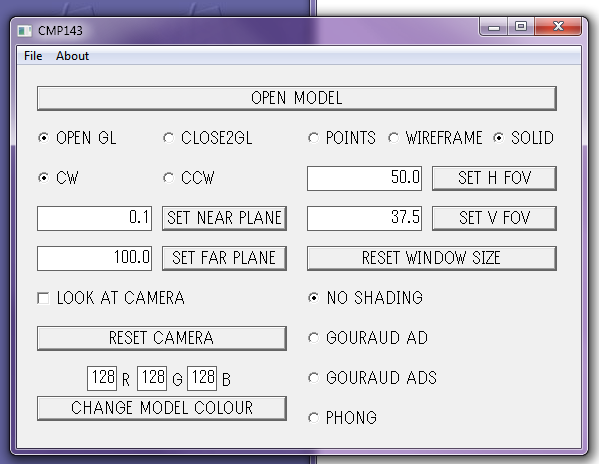
\includegraphics[scale=0.5]{1.png}
\end{center}
\begin{itemize}
\item[1.] Close2GL part
\begin{itemize}
\item[a)] Points\\
The interface has a toggle for the user to choose to see the model as points, wireframe or as a solid. This functionality works both for OpenGL and Close2GL, as shown below:
\begin{center}
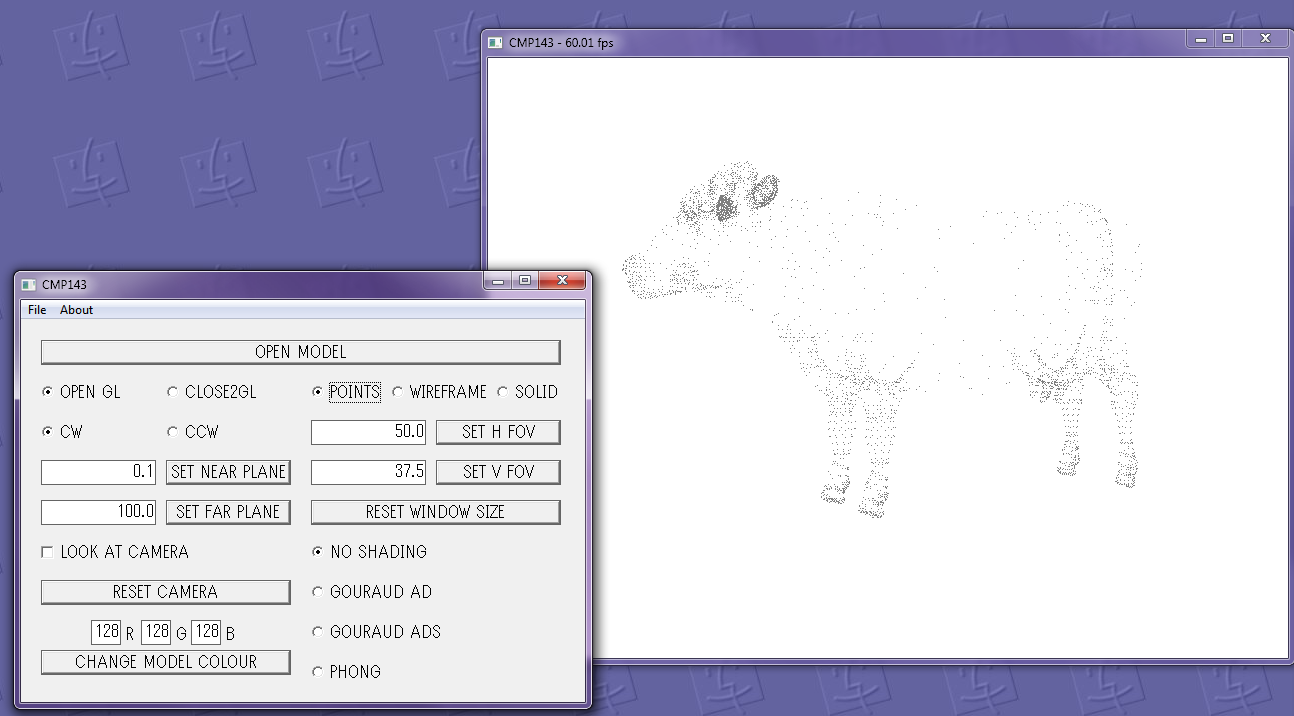
\includegraphics[scale=0.4]{2.png}
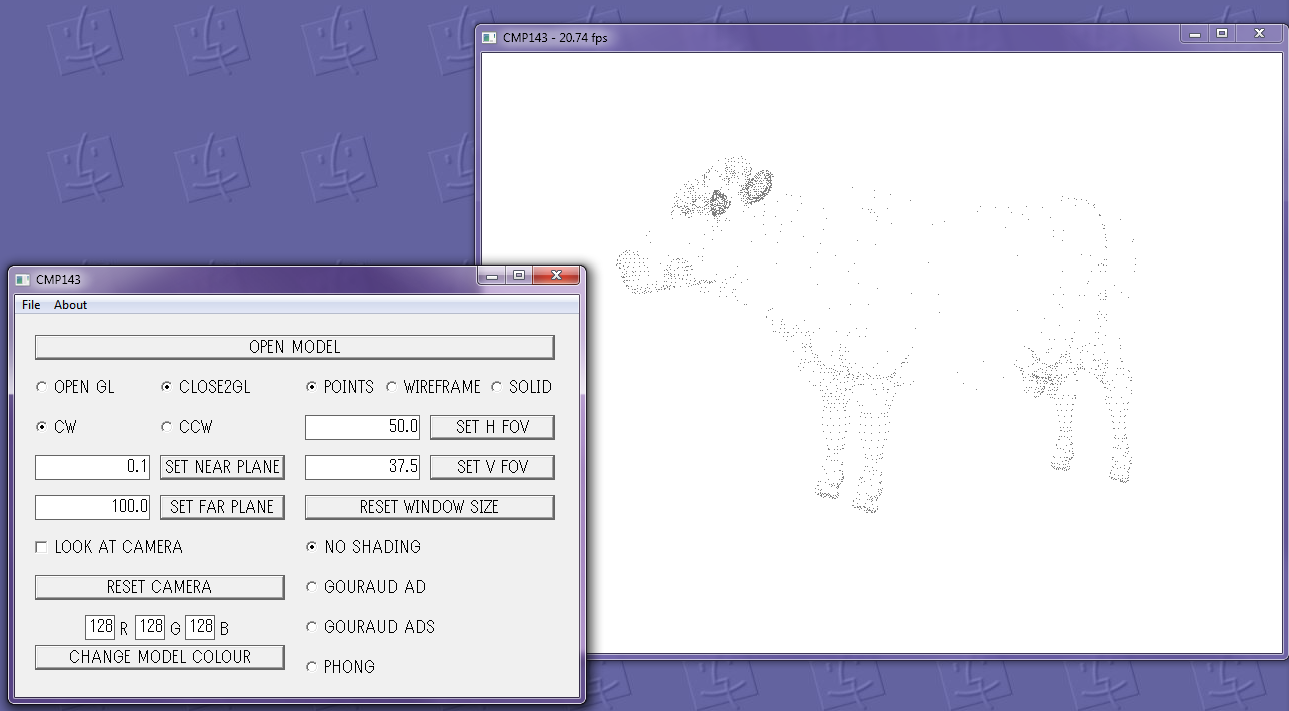
\includegraphics[scale=0.4]{3.png}
\end{center}
As it can be seen comparing the two pictures above, the Close2GL shows fewer points. This is the case because of the backface culling done to discard the vertices in which the fragment normals face away from the camera.
\item[b)] Wireframe\\
When the toggle is set to ``Wireframe'', these are the results obtained:
\begin{center}
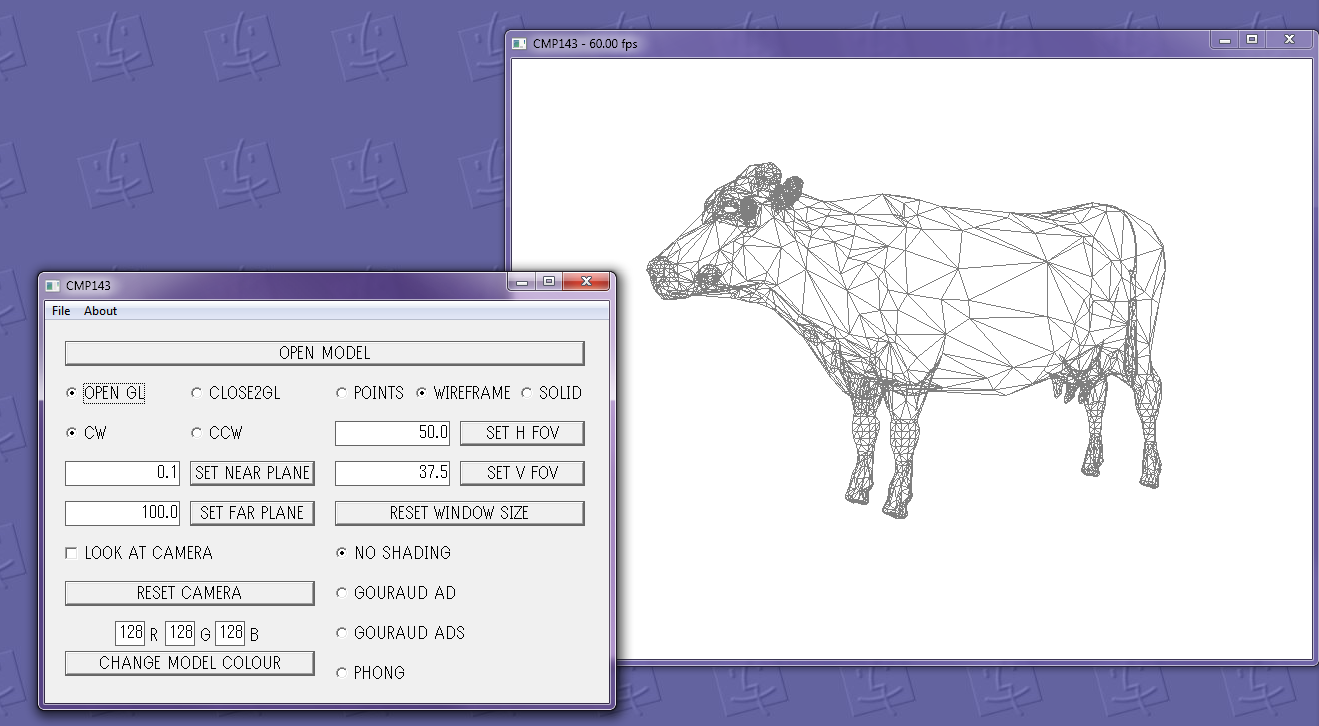
\includegraphics[scale=0.4]{4.png}
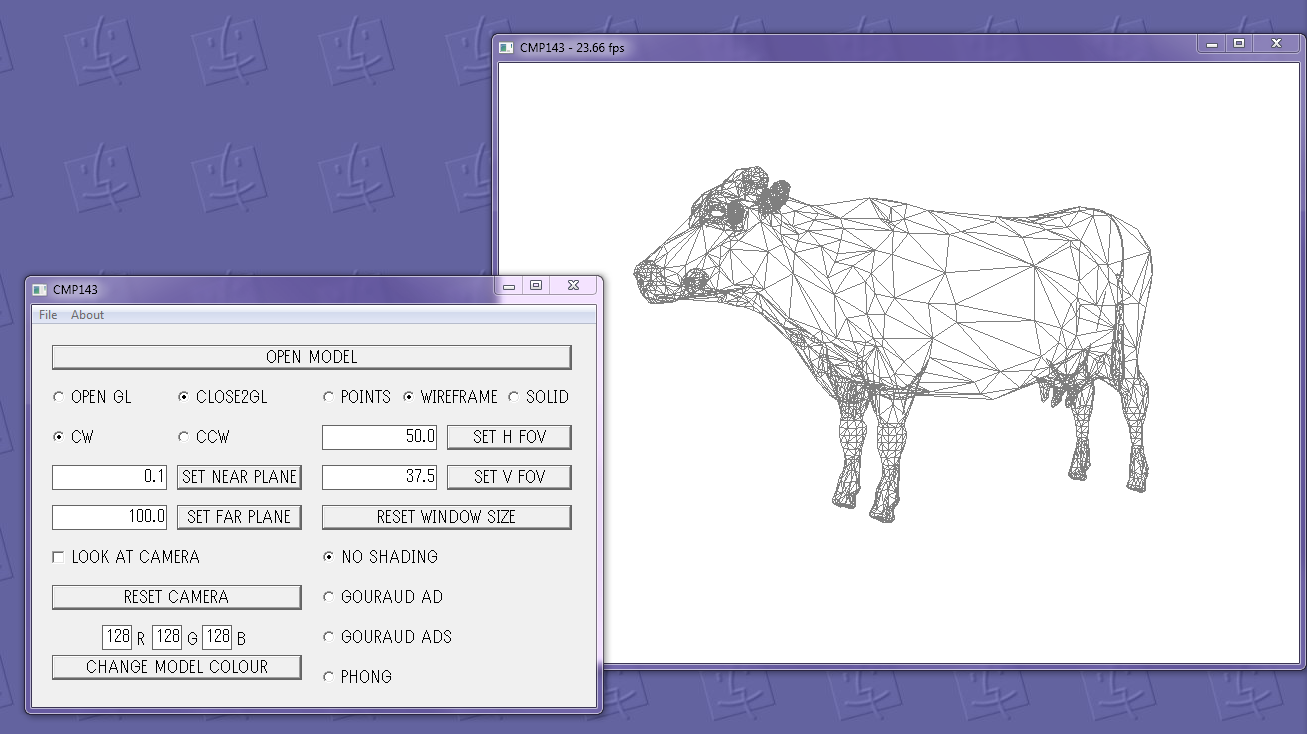
\includegraphics[scale=0.4]{5.png}
\end{center}
\item[c)] Solid\\
When the toggle is set to ``Solid'', these are teh results obtained:
\begin{center}
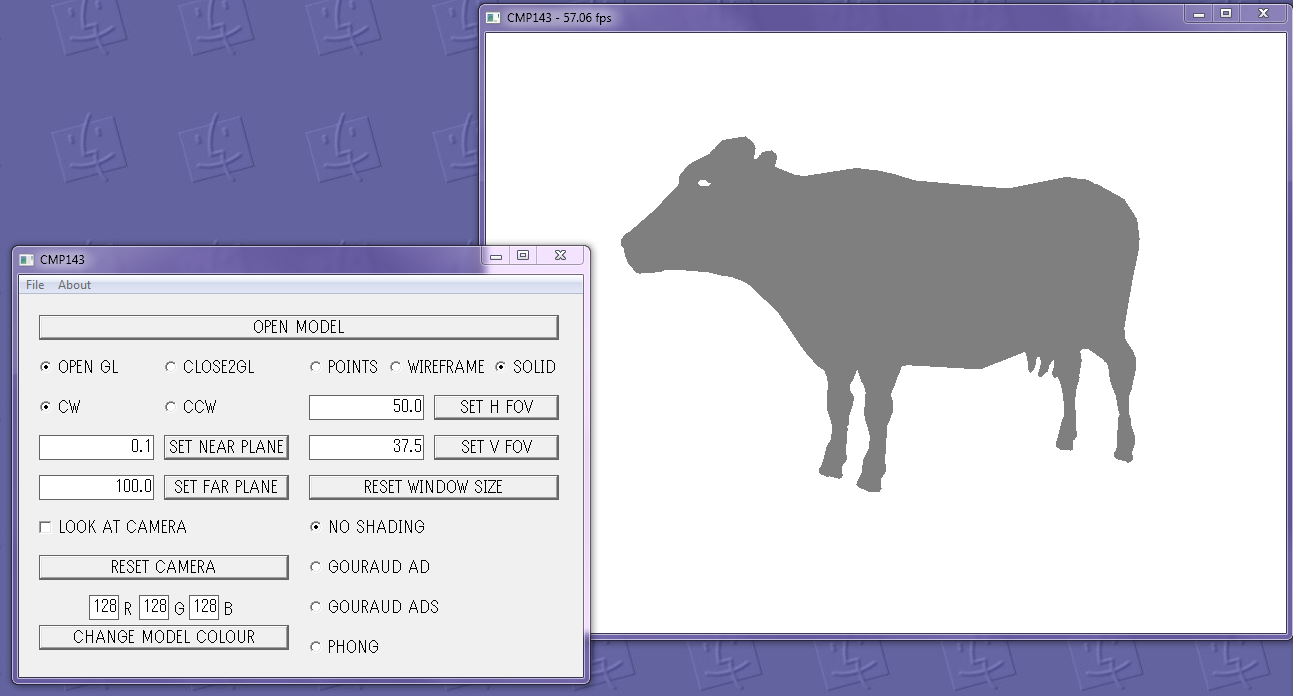
\includegraphics[scale=0.4]{6.png}
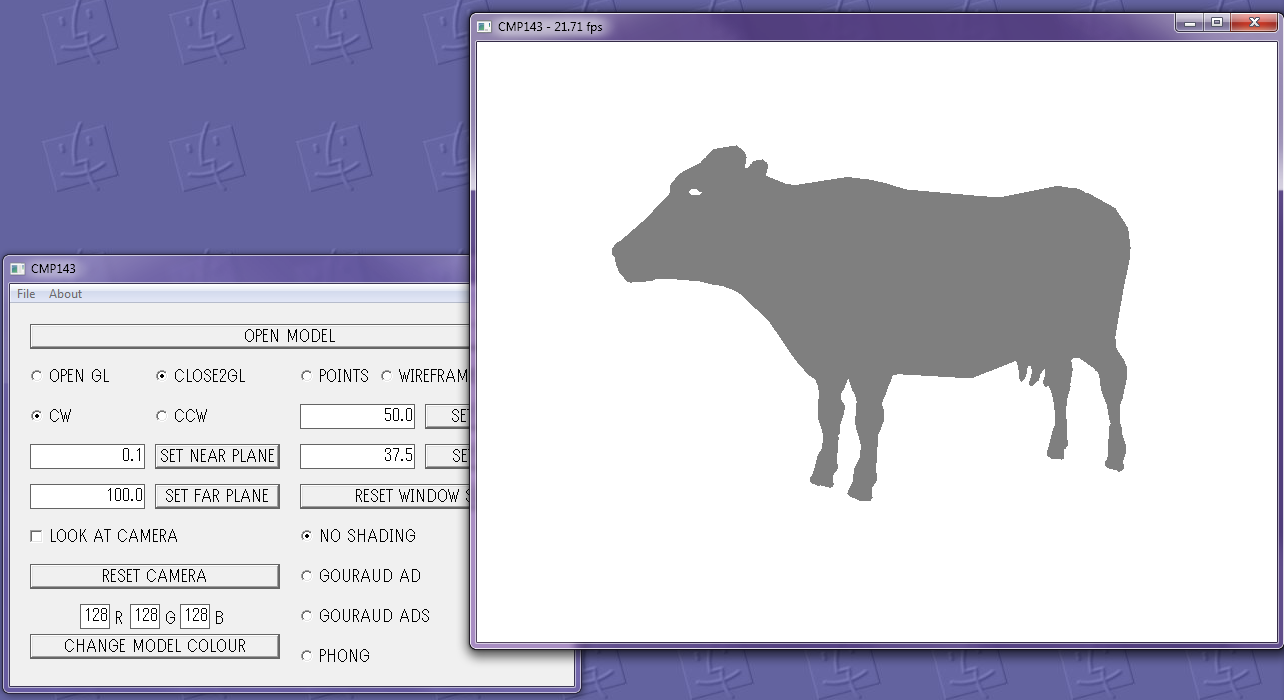
\includegraphics[scale=0.4]{7.png}
\end{center}

\item[d)] Translation\\
The Close2GL implementation supports translation as well, compare the following two images, of the start position (first image) and the image after a translation on the X-axis (second image).
\begin{center}
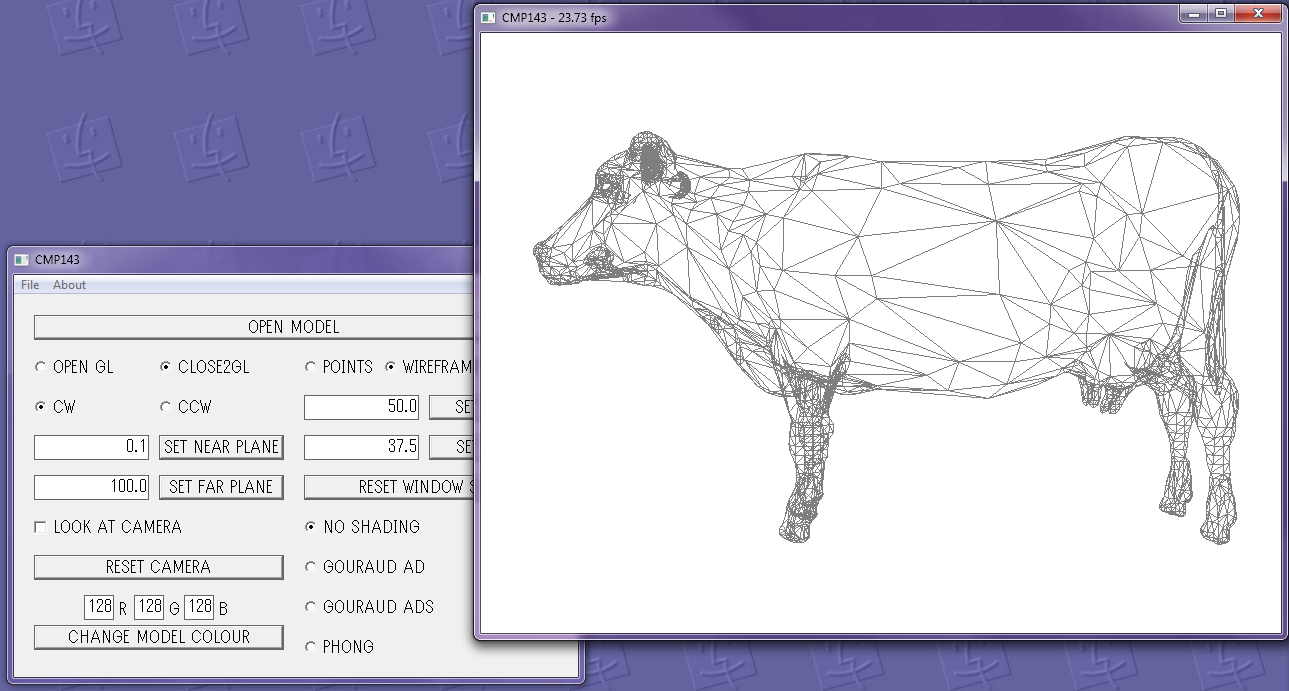
\includegraphics[scale=0.4]{8.png}
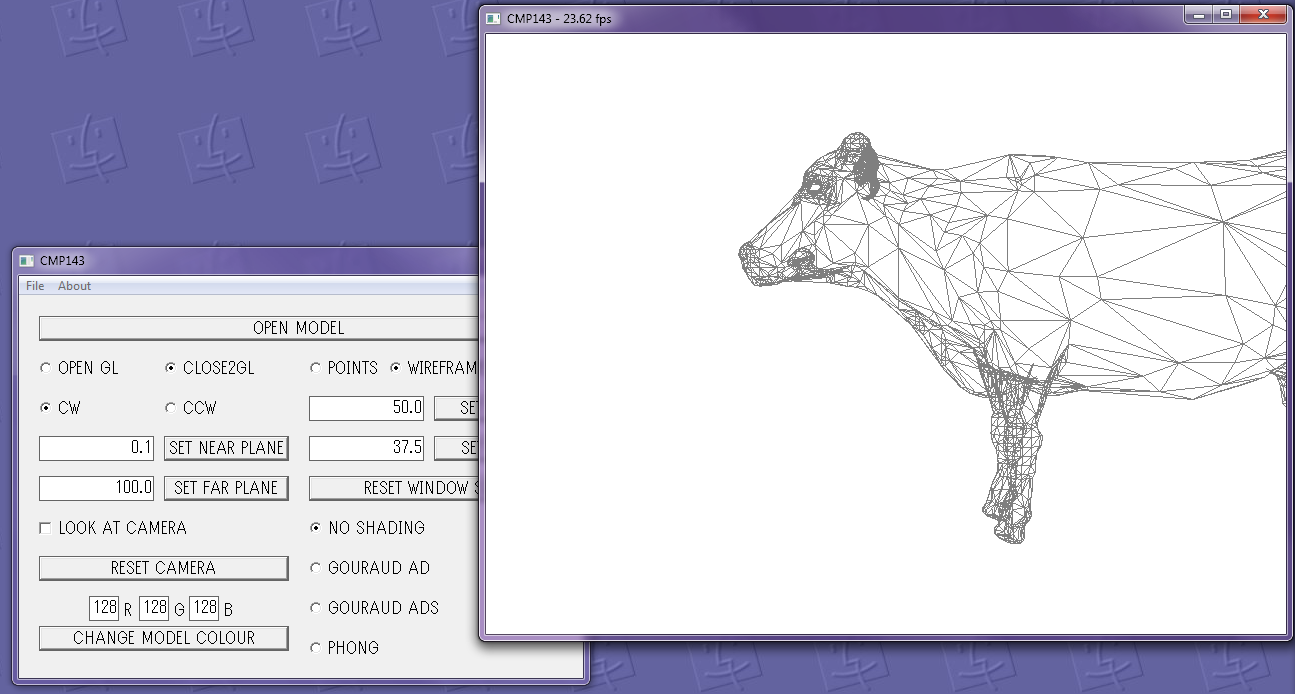
\includegraphics[scale=0.4]{9.png}
\end{center}

\item[e)] Supports translation while keeping fixed look at point?\\
If ``Look at Camera'' is selected, the camera will translate while also keeping fixed at the point in the center of the object, as shown below:
\begin{center}
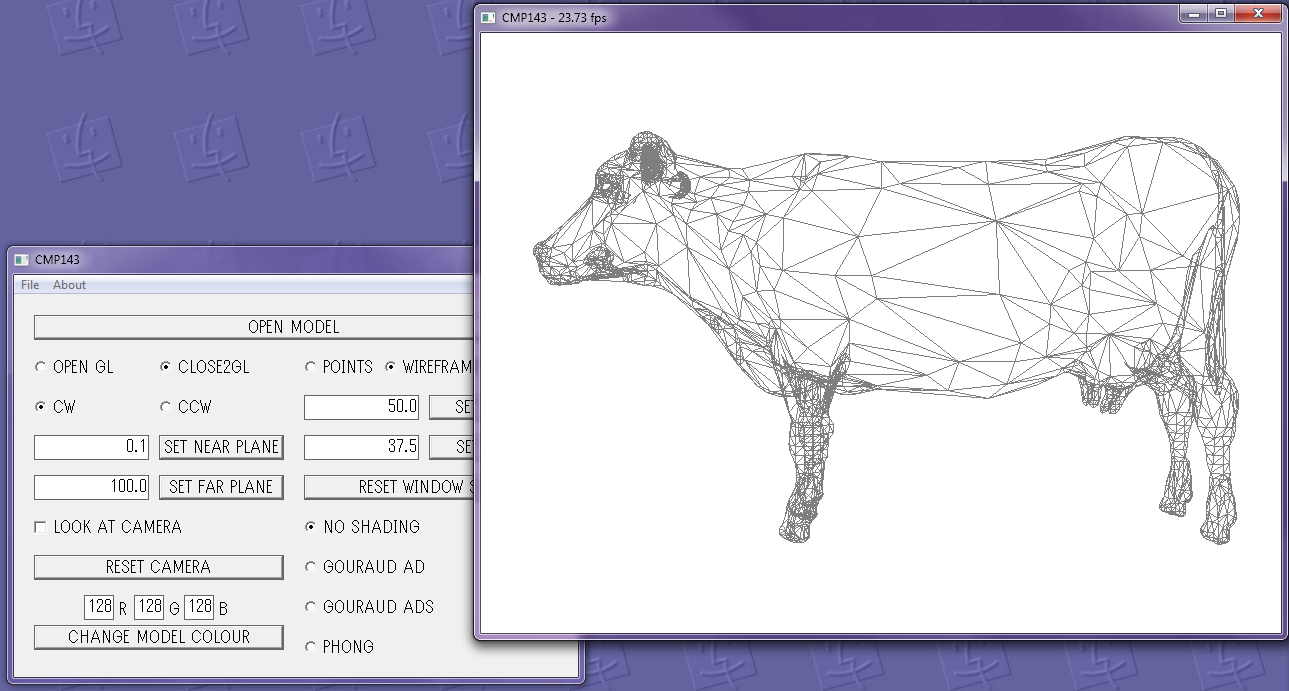
\includegraphics[scale=0.4]{8.png}
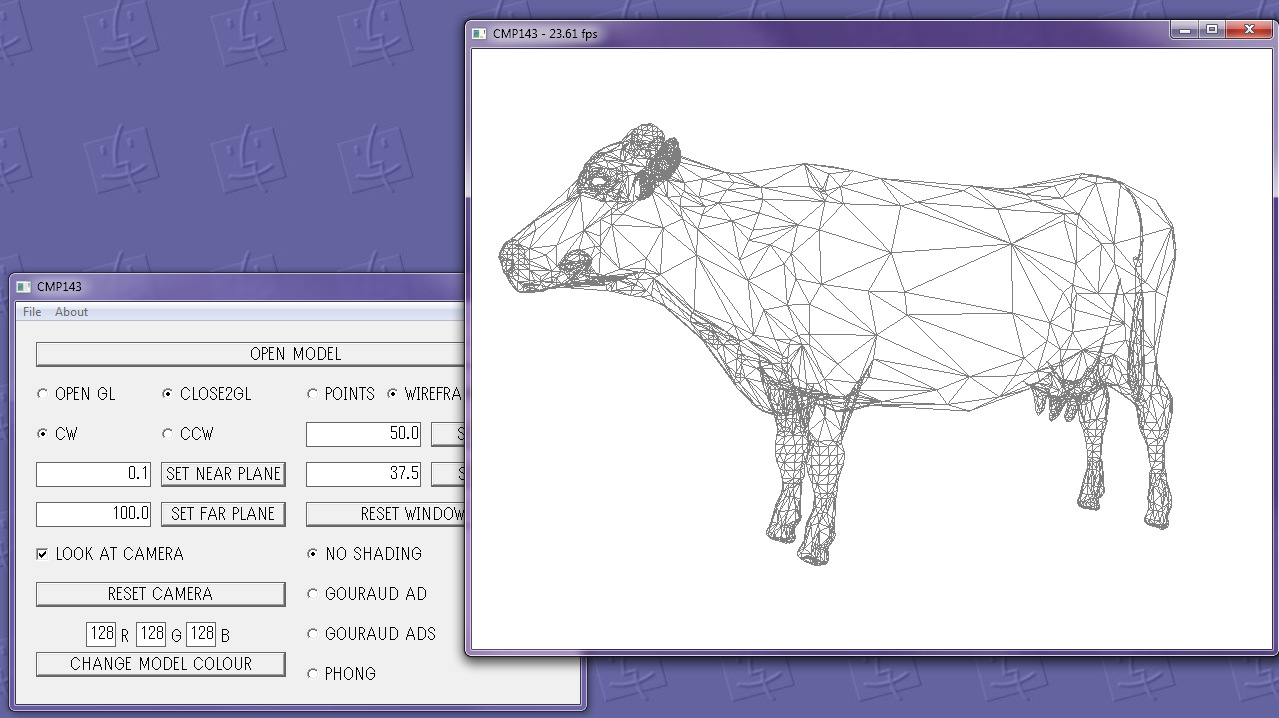
\includegraphics[scale=0.4]{10.png}
\end{center}

\item[f)] Rotation\\
Rotation is also supported, as shown below:
\begin{center}
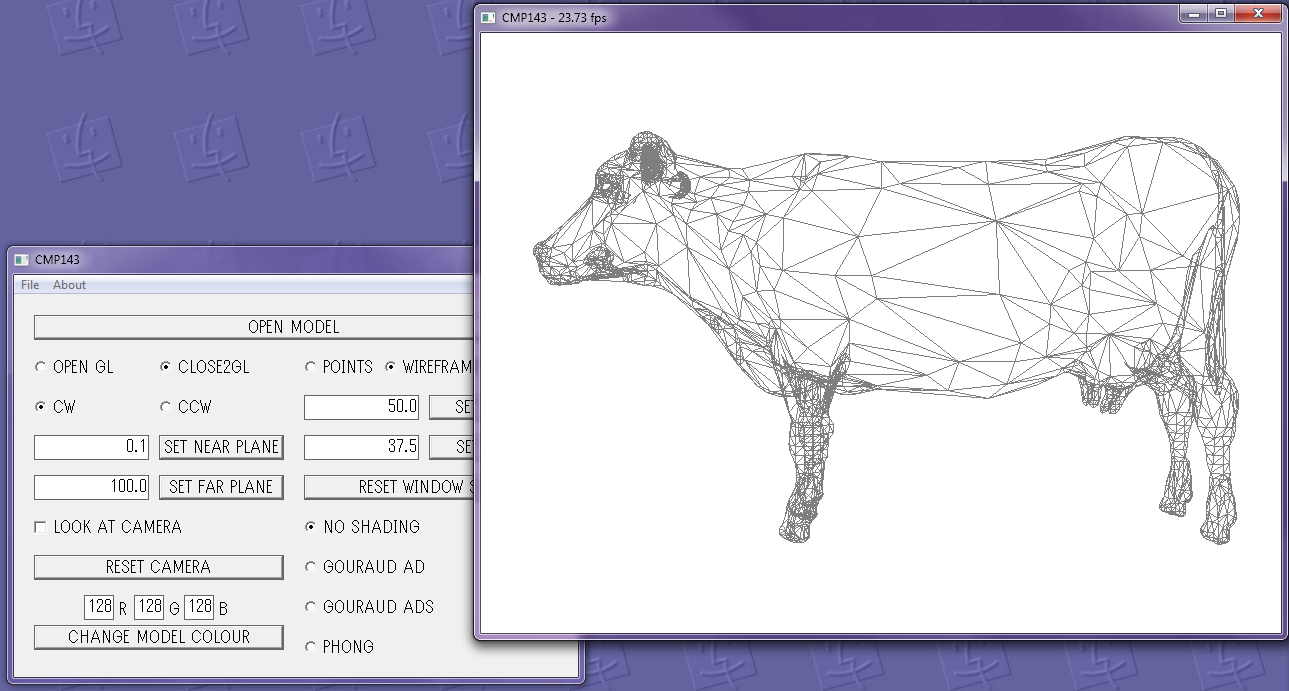
\includegraphics[scale=0.4]{8.png}
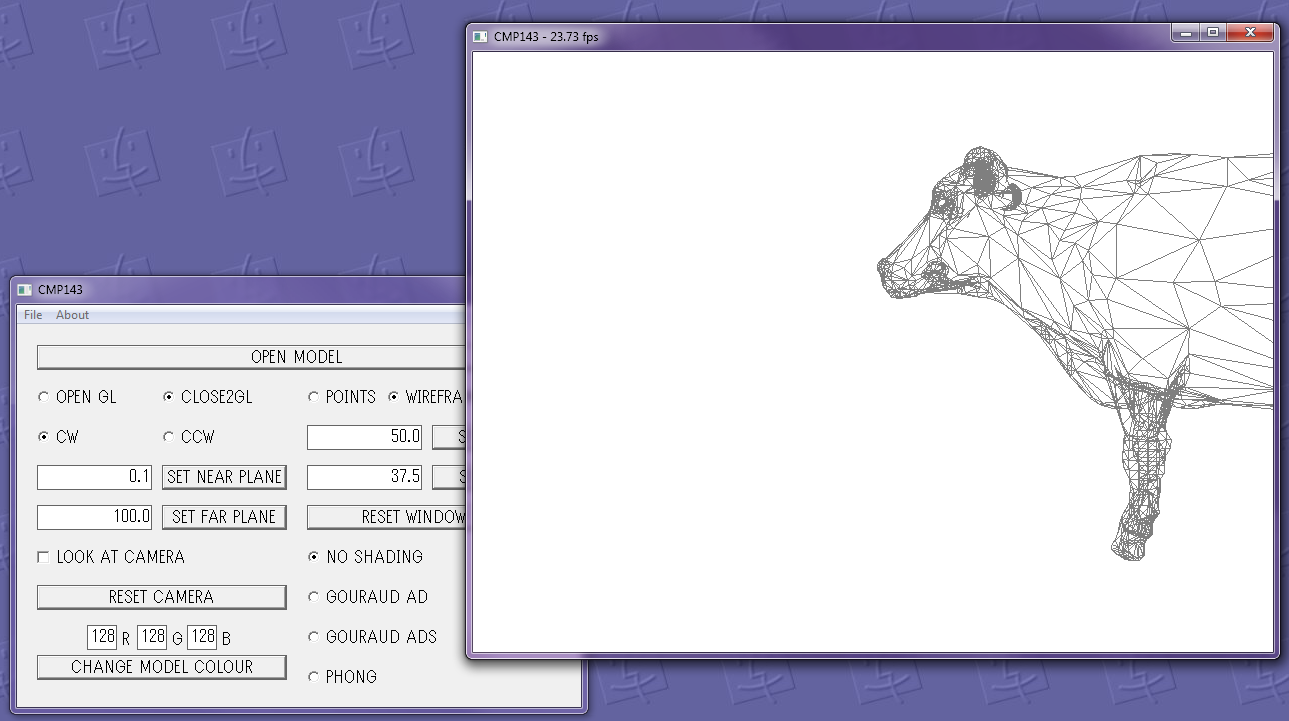
\includegraphics[scale=0.4]{11.png}
\end{center}

\item[g)] Backface culling\\
As seen on item 1.a), backface culling is performed to not send the vertices belonging to fragments that would be faced away from the camera to the GPU to render. The source code is included with this report and the implementation can be found on the \texttt{GLuint BuildTriangles(ModelObject model)} function. 

\item[h)] Discarding vertices behind or on the same plane as the camera\\
This was also implemented on the \texttt{GLuint BuildTriangles(ModelObject model)} function from the \texttt{main.cpp} file.

\item[i)] Change Hfov\\
This is supported, and the results are shown below:
\begin{center}
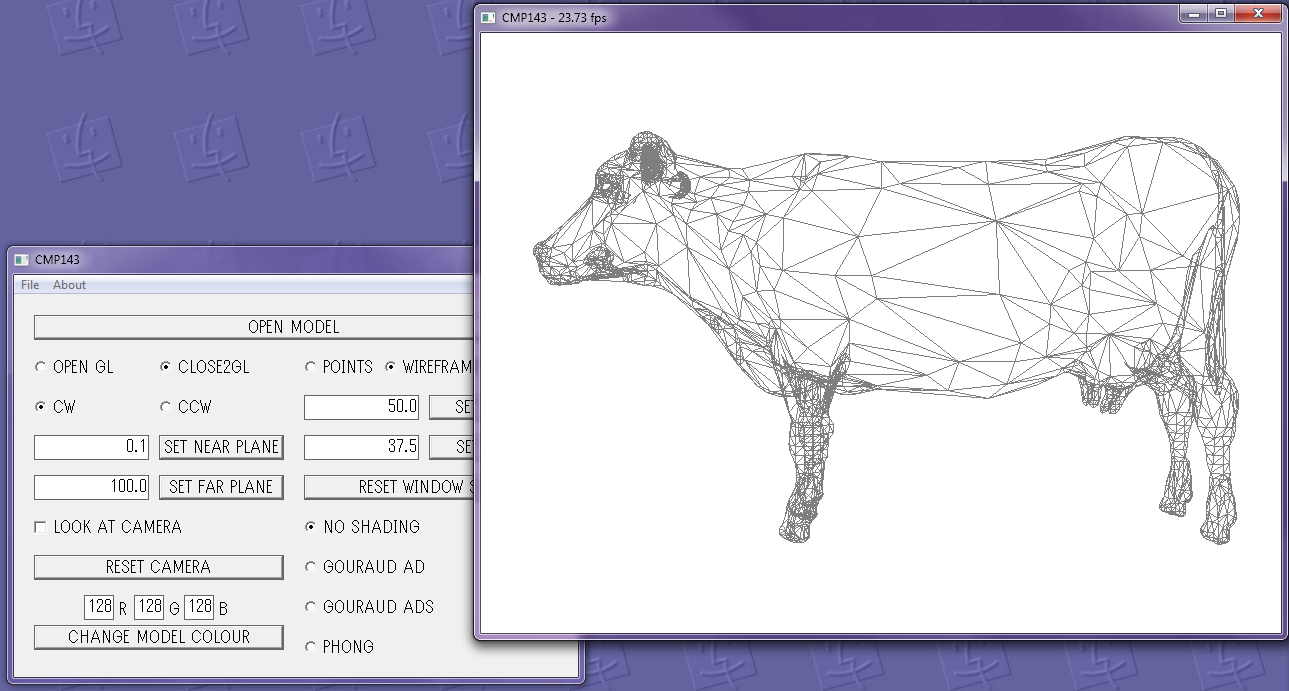
\includegraphics[scale=0.4]{8.png}
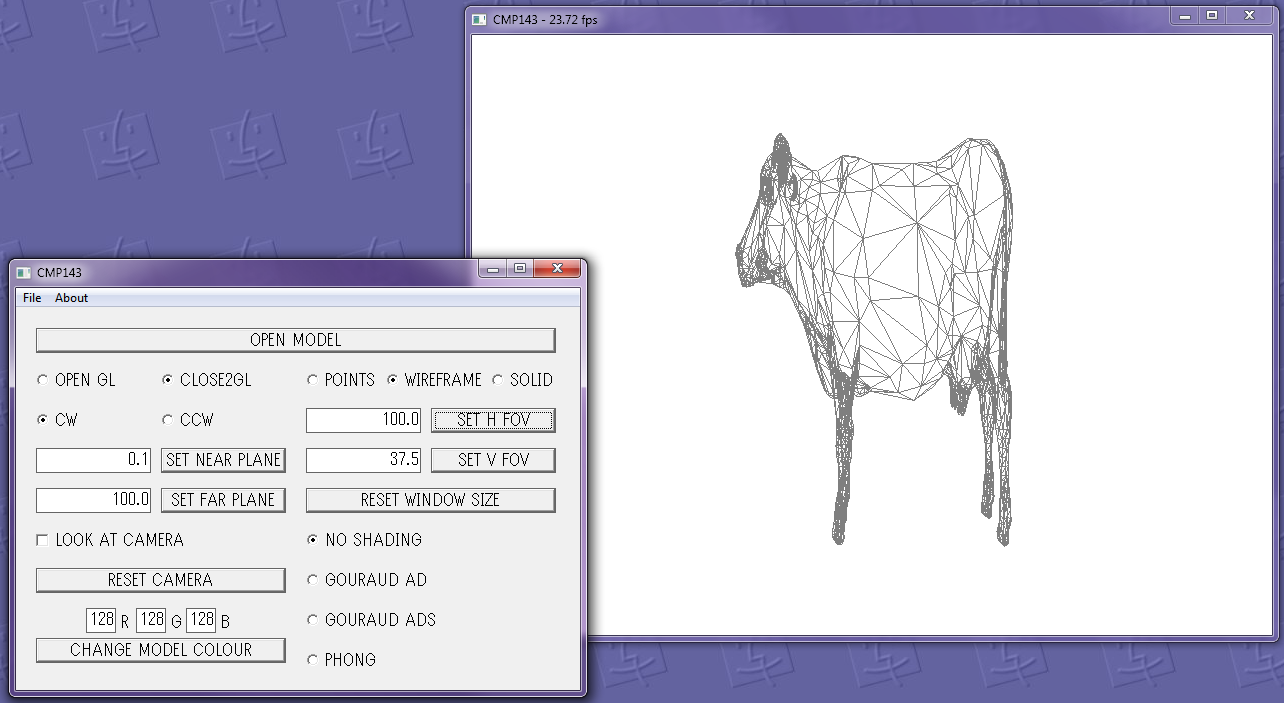
\includegraphics[scale=0.4]{12.png}
\end{center}
In this case, the Horizontal FOV was changed from 50° (base value) to 100°. The image looks squished horizontally due to that.

\item[j)] Change Vfov\\
This is also supported, and the results are shown below:
\begin{center}
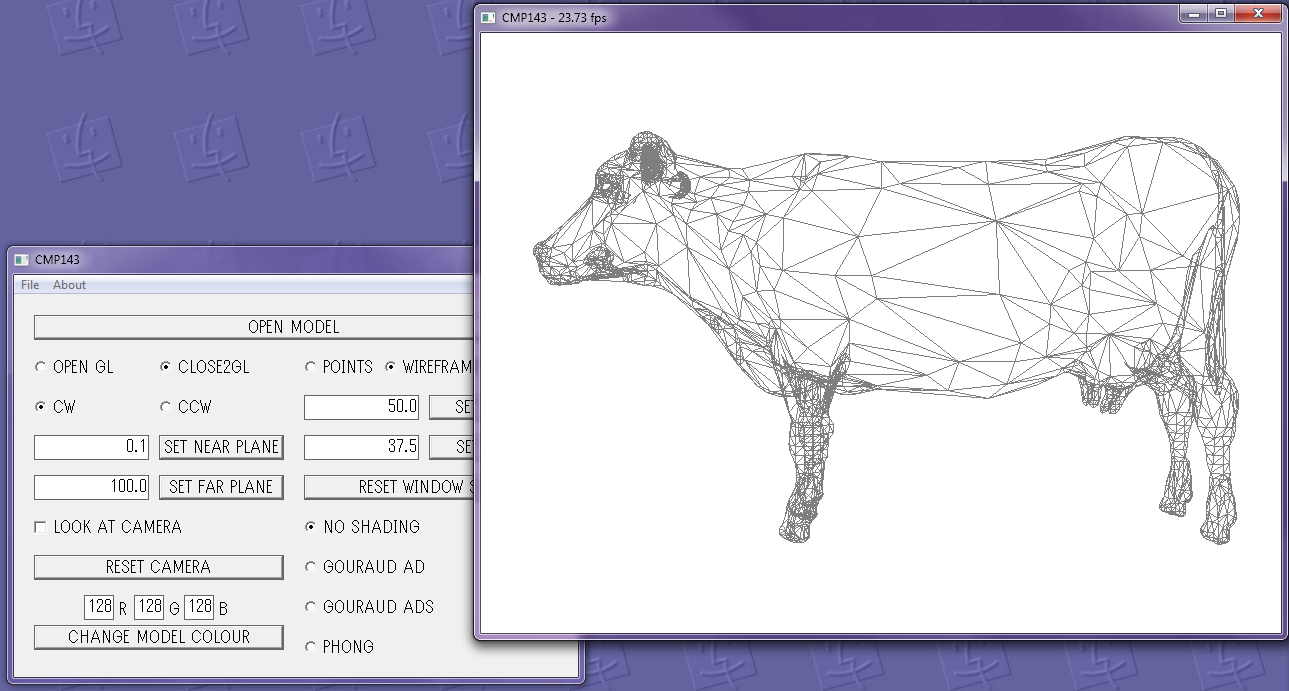
\includegraphics[scale=0.4]{8.png}
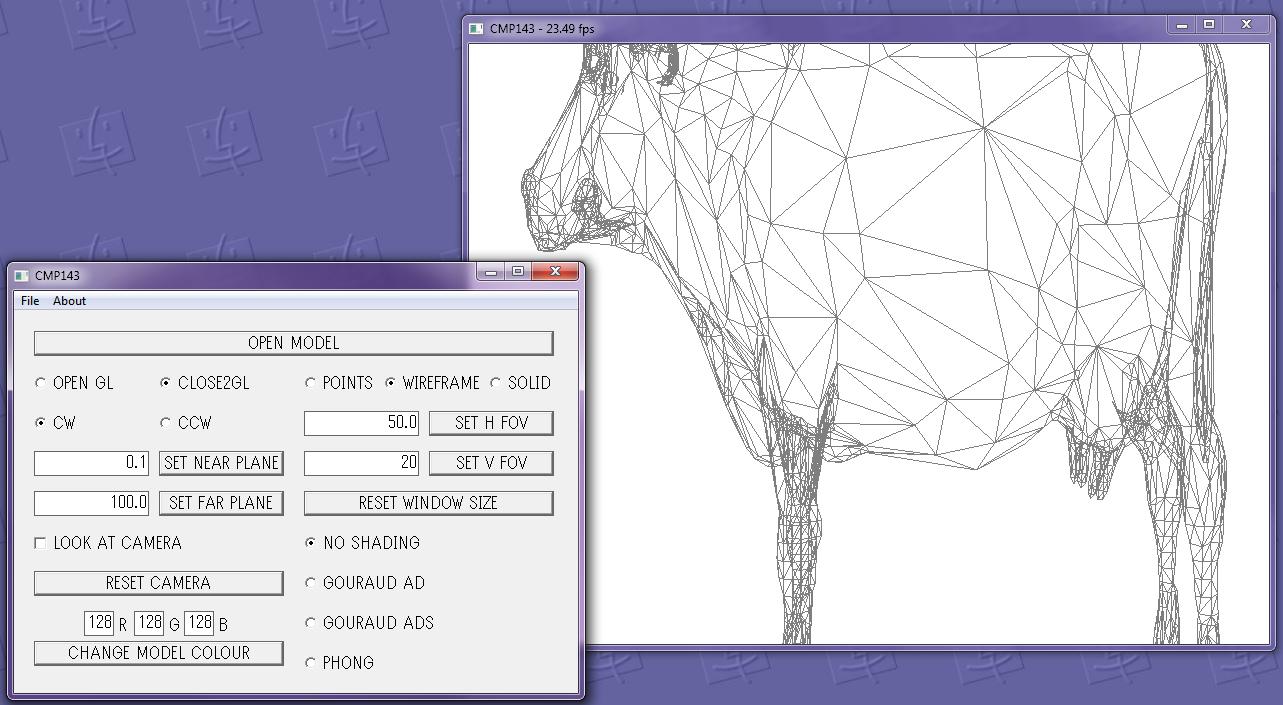
\includegraphics[scale=0.4]{13.png}
\end{center}
In this case, the Vertical FOV was changed from 37.5° (base value) to 20°. The image looks stretched vertically due to that.

\item[k)] Works after the window has been resized?\\
This is supported, and the results from changing the window size from the default 800x600 size to having fewer horizontal pixels is shown below:
\begin{center}
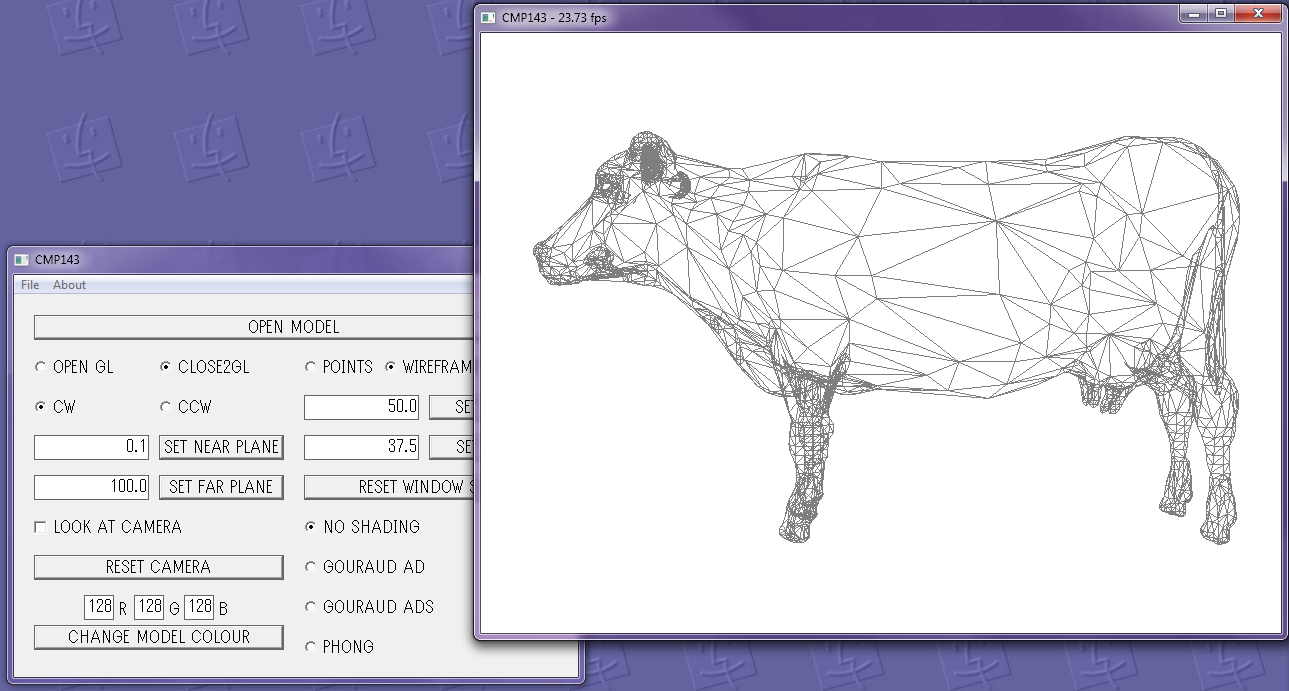
\includegraphics[scale=0.4]{8.png}
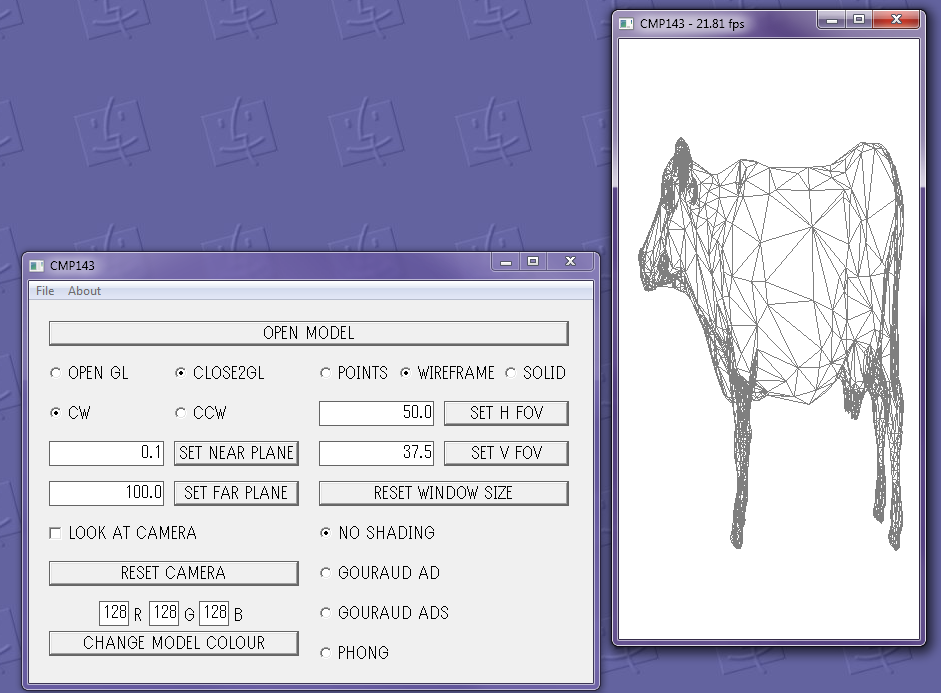
\includegraphics[scale=0.4]{14.png}
\end{center}
\end{itemize}

\item[2.] Renderings from OpenGL and Close2GL are synchronized?\\
As shown on items 1.a), 1.b), and 1.c), the OpenGL/Close2GL toggle can be switched without affecting the position of the vertices shown. With the exception of the points mode, in which OpenGL seems to (incorrectly) show, in that mode, vertices that would be otherwise removed by backface culling, the visualizations are identical to each other.

\item[3.] OpenGL part\\
In OpenGL mode, the shaders were implemented and can be selected with the shader toggle on the bottom right of the interface.
\begin{itemize}
\item[a)]Gouraud Shading AD\\
This is the result obtained with Gouraud Shading AD:
\begin{center}
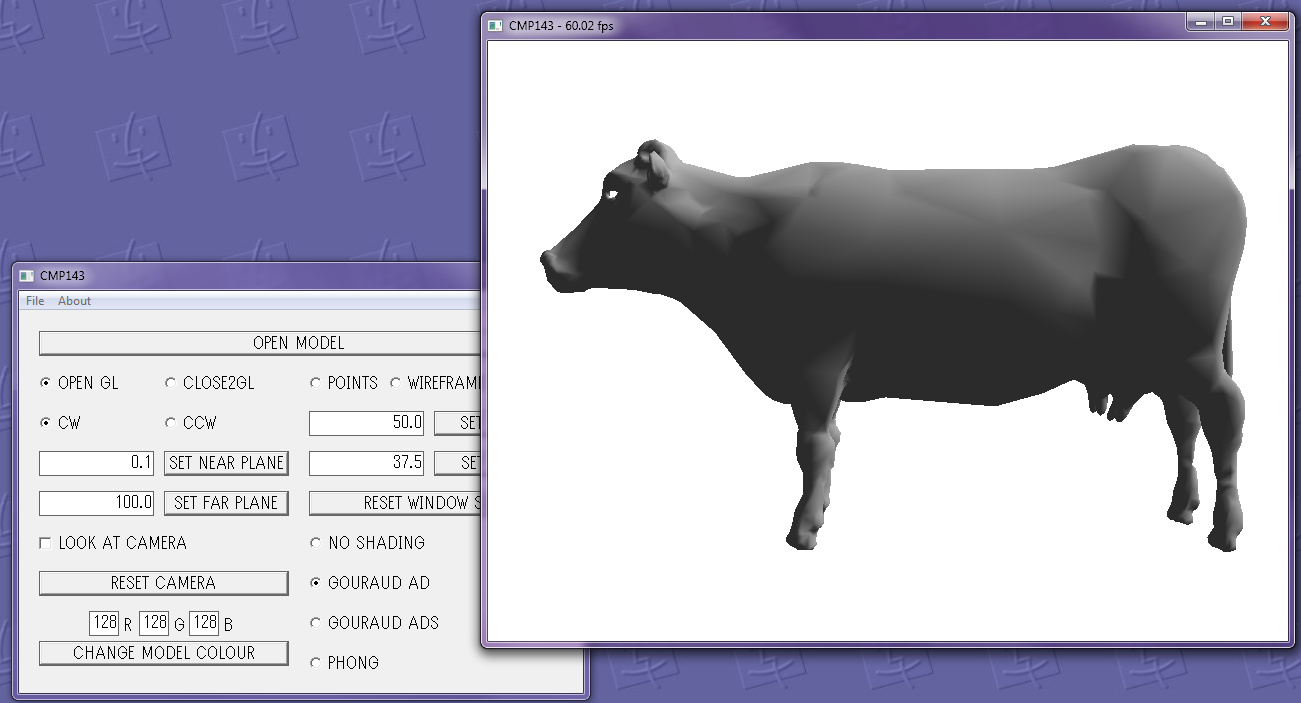
\includegraphics[scale=0.4]{15.png}
\end{center}
\item[b)] Gouraud Shading ADS\\
This is the result obtained with Gouraud Shading ADS:
\begin{center}
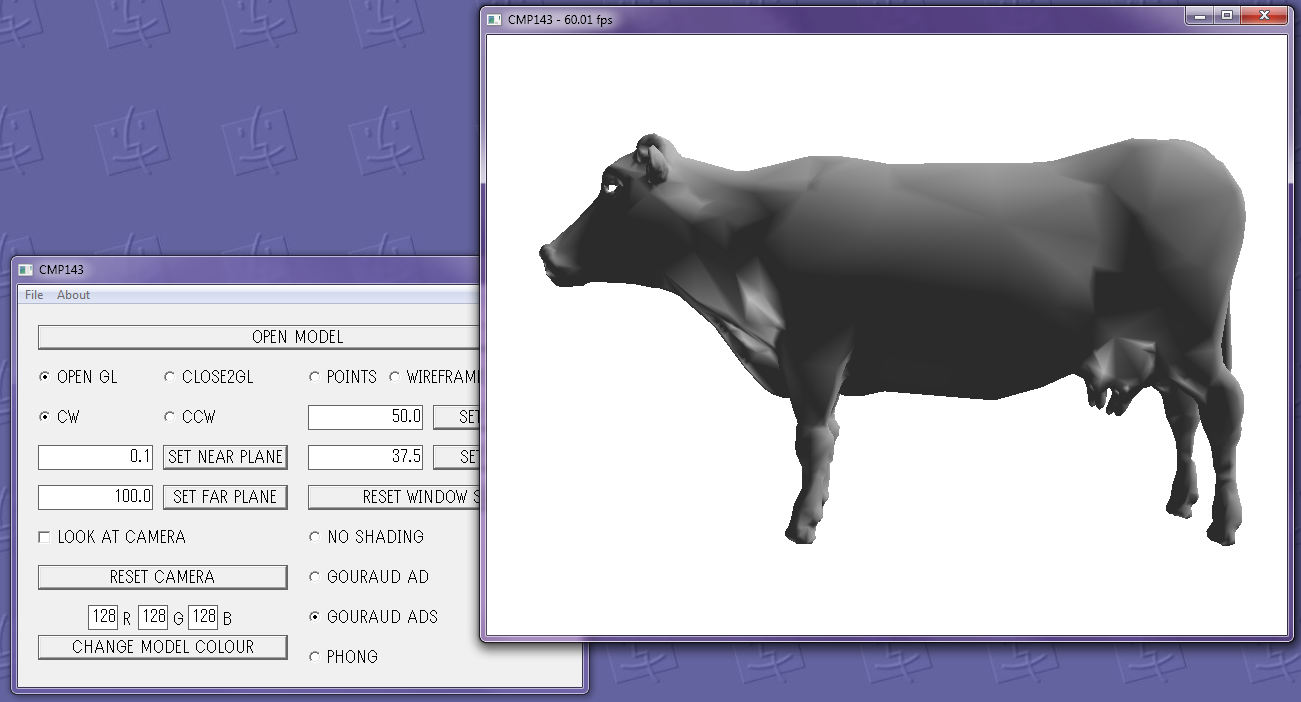
\includegraphics[scale=0.4]{16.png}
\end{center}
\item[c)] Phong Shading\\
This is the result obtained with Phong Shading:
\begin{center}
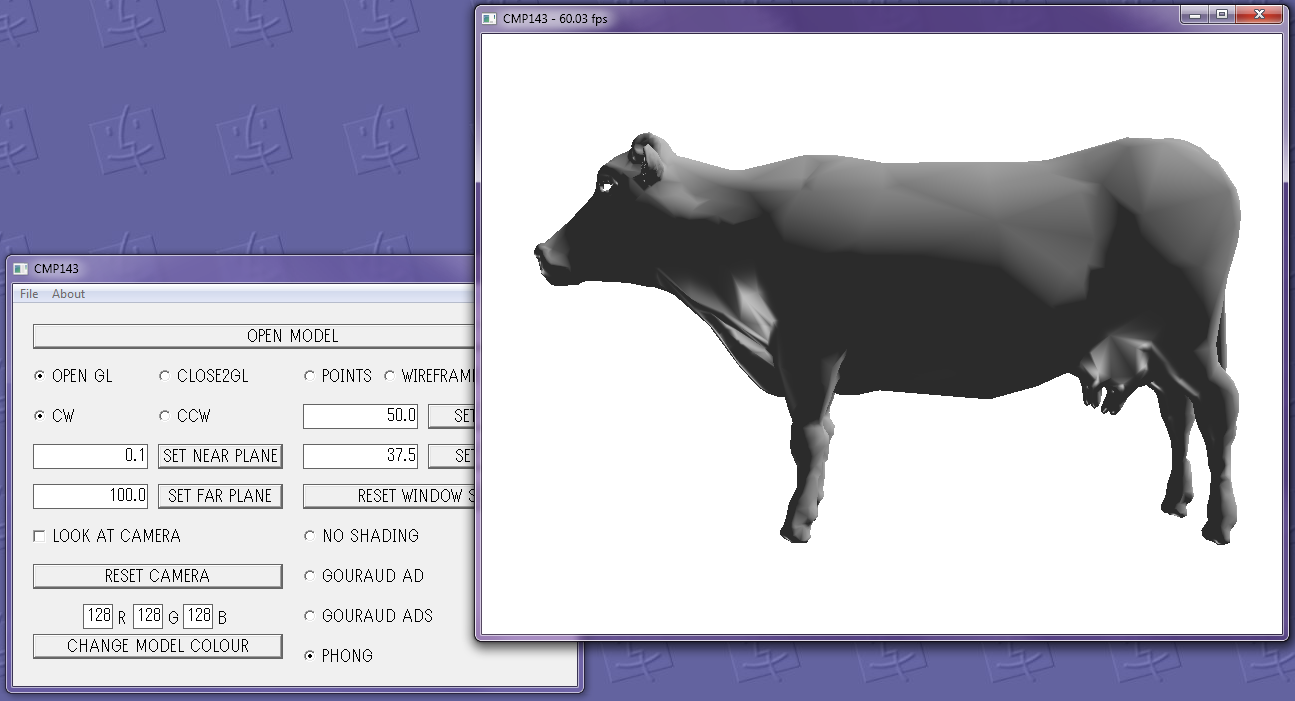
\includegraphics[scale=0.4]{17.png}
\end{center}
\item[d)] Use of Subroutines\\
As it can be seen in the \texttt{triangles.frag} and \texttt{triangles.vert} files, subroutines were implemented in both the fragment and vertex shaders to select the desired shader with the information sent from the interface.
\end{itemize}
\item[4.] FPS rate\\
The FPS rate is shown on the title of the OpenGL window, on the top left corner, next to the name of the program.
\begin{center}
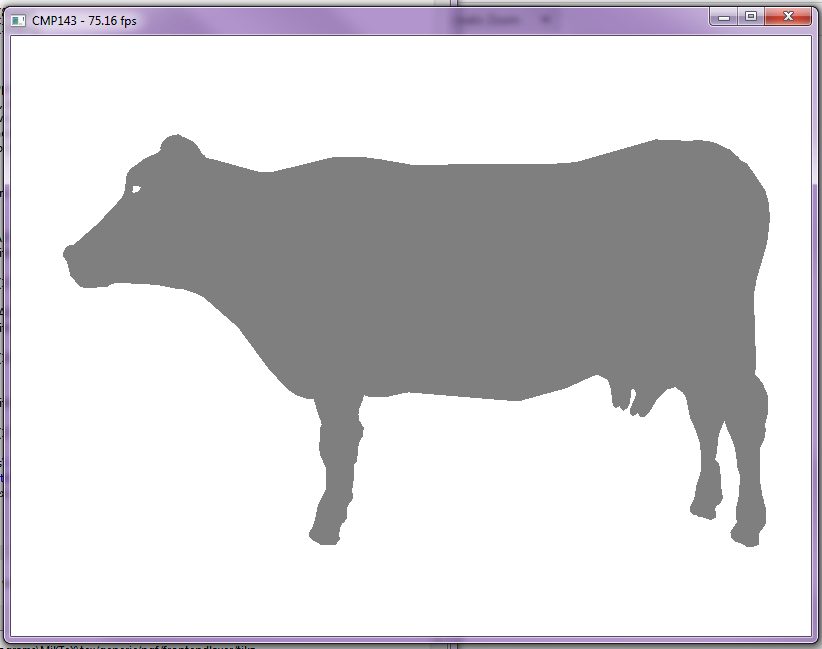
\includegraphics[scale=0.4]{18.png}
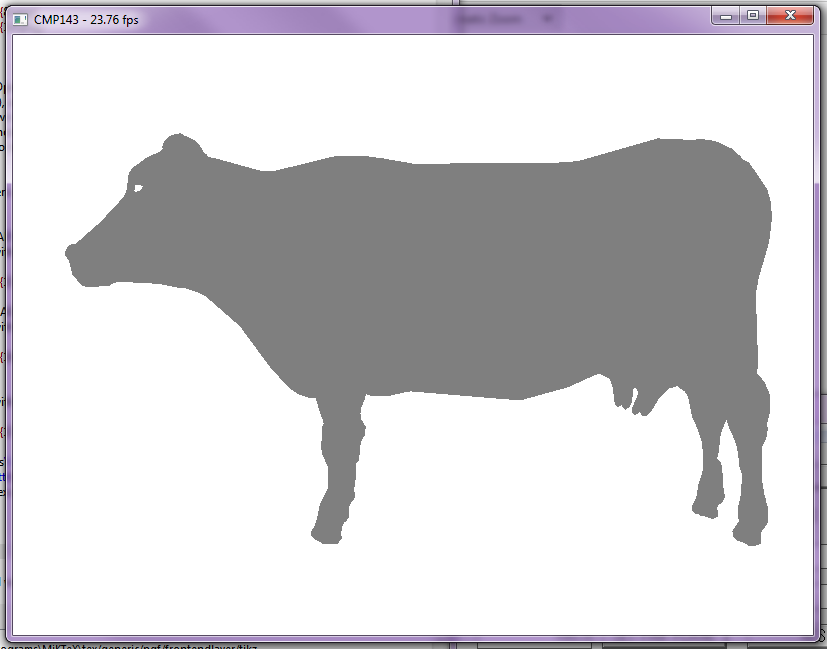
\includegraphics[scale=0.4]{19.png}
\end{center}
The first image shows the frame rate with OpenGL, it is capped at around 75 fps, the frequency of the monitor currently being used. The second image shows the frame rate using Close2GL, which is at about 23 fps, as it can be seen some performance is lost while doing all the transformations in the CPU instead of doing it on the GPU.
\end{itemize}

The source code is included with this report.

\end{document}